\documentclass[12pt]{article}
\usepackage{listings}
\usepackage{enumerate}
\usepackage{xcolor}
\usepackage{graphicx}
\usepackage{booktabs}
\usepackage[italian]{babel}
\usepackage[utf8]{inputenc}
\usepackage{float}
\usepackage{caption}
\usepackage[shortlabels]{enumitem}
\usepackage[T1]{fontenc}

\usepackage{mathpazo} 

\definecolor{codeblue}{rgb}{0.21, 0.46, 0.80}
\definecolor{backcolour}{rgb}{0.95,0.95,0.92}
\definecolor{monokai@black}{HTML}{2C2C2A}
\definecolor{monokai@gray}{HTML}{524F52}
\definecolor{monokai@magenta}{HTML}{D33682}
\definecolor{monokai@blue}{HTML}{004C99}

\lstdefinestyle{sql}{
	frame=tb,
	language=SQL,
	backgroundcolor=\color{backcolour},
	aboveskip=3mm,
	belowskip=3mm,
	showstringspaces=false,
	columns=flexible,
	basicstyle={\small\ttfamily},
	numbers=left,
	numberstyle=\tiny\color{monokai@black},
	numbersep=5pt,
	stepnumber=2,
	breaklines=true,
	breakatwhitespace=true,
	tabsize=3,
	numberstyle=\color{monokai@gray},
	keywordstyle=\color{codeblue},
	stringstyle=\color{monokai@magenta}\ttfamily,
	identifierstyle=\color{monokai@black},
	commentstyle=\color{monokai@blue},
	emphstyle=\color{monokai@red},
	columns=fullflexible
}

\newcommand{\sectionline}[2]{%
  \nointerlineskip \vspace{.5\baselineskip}\hspace{\fill}
  {\color{#1}
    \resizebox{0.5\linewidth}{2ex}
    {{%
    {\begin{tikzpicture}
    \node  (C) at (0,0) {};
    \node (D) at (9,0) {};
    \path (C) to [ornament=#2] (D);
    \end{tikzpicture}}}}}%
    \hspace{\fill}
    \par\nointerlineskip \vspace{.5\baselineskip}
}

\renewcommand{\lstlistingname}{Codice}

\begin{document}
\begin{titlepage}
	\newcommand{\HRule}{\rule{\linewidth}{0.5mm}}

	\center
	
	\textsc{\LARGE Università degli studi di Firenze}\\[1.5cm] 
	
	\textsc{\Large Curriculum Data Science}\\[0.5cm] 
	
	\textsc{\large Data mining and organisation}\\[0.5cm] 

	\HRule\\[0.4cm]
	
	{\huge\bfseries Analisi carriere studenti iscritti al I anno del corso di laurea in Informatica}\\[0.4cm] % Title of your document
	
	\HRule\\[1.5cm]
	\vfill\vfill\vfill 

	\begin{minipage}{\textwidth}
		\begin{flushright}
			\large
			\textit{Studenti}\\
			Tommaso \textsc{Ceccarini}\\
			\texttt{tommaso.ceccarini1@stud.unifi.it}\\
			Filippo \textsc{Mameli}\\
			\texttt{filippo.mameli@stud.unifi.it}
		\end{flushright}
	\end{minipage}
	
	\vfill
	
	{\large\today}
	
\end{titlepage}

\newpage

\tableofcontents

\newpage

\thispagestyle{empty}\clearpage\mbox{}\clearpage

\section{Descrizione dati iniziali}
Il dataset che abbiamo analizzato contiene dati sulle carriere accademiche degli studenti del corso di laurea di informatica dell'università degli studi di Firenze e il loro voto conseguito 
al test di ingresso. 
In particolare, le informazioni presenti sono:
\begin{itemize}
	\item Coorte: Anno di immatricolazione
	\item Crediti totali: Numero crediti complessivi dello studente
	\item Crediti con voto: Numero di crediti assegnati allo studente per esami con votazione in trentesimi(tutti tranne Inglese)
	\item Voto medio: Media pesata dei voti degli esami sostenuti
\end{itemize}
In seguito ci sono sei coppie di attributi che indicano:
\begin{itemize}
	\item Nome dell'esame
	\item Data in cui lo studente ha sostenuto l'esame
\end{itemize}
Gli esami sono Algoritmi e strutture dati (ASD), Architetture degli elaboratori(ARC), Programmazione(PRG), Analisi I(ANI), Matematica discreta e logica(MDL) e Inglese.
\begin{itemize}
	\item Punteggio conseguito al test di ingresso.
\end{itemize}
Per quanto riguarda gli attributi relativi ai voti degli esami i valori che questi assumono sono:
il voto conseguito dallo studente nel caso in cui abbia sostenuto l'esame oppure
zero se lo studente non ha sostenuto l'esame durante la sessione estiva del proprio anno di immatricolazione.
\section{Gestione dei dati}
Abbiamo deciso di effetture le seguenti operazioni sul dataset:
\begin{itemize}
	\item eliminazione degli studenti che hanno sostenuto solo inglese
	\item riportare tutti gli attributi relativi alle date degli esami nel formato YYYY-MM-DD
\end{itemize}

Il motivo per cui abbiamo deciso di eseguire l'operazione del primo punto è che gli studenti in questione non avendo voti in trentesimi non ci sono parsi particolarmente significativi per analisi.

Per quanto riguarda il secondo punto invece, nel caso in cui uno studente non avesse sostenuto un particolare esame, erano presenti valori pari a zero in alcuni casi e valori pari a ``0000-00-00'' in altri.
Abbiamo quindi deciso di trattare questa incosisistenza dei dati ponendo i valori pari a ``0000-00-00''.

Per effetturare queste due operazioni abbiamo importato il dataset in un database creando per prima una tabella, che è stata popolata in seguito importando il file CSV con i comandi riportati in Codice \ref{import}.
\begin{lstlisting}[caption={Creazione della table}, style=sql, label={import}, captionpos=b]
CREATE TABLE 'studenti' (
  'coorte' int(11),
  'crediti_totali' int(11),
  'crediti_con_voto' int(11),
  'voto_medio' int(11),
  'ASD' int(11),
  'data_ASD' text,
  'ARC' int(11),
  'data_ARC' text,
  'PRG' int(11),
  'data_PRG' text,
  'ANI' int(11),
  'data_ANI' text,
  'MDL' int(11),
  'data_MDL' text,
  'INGLESE' int(11),
  'data_INGLESE' text,
  'TEST' int(11)
) ENGINE=InnoDB

LOAD DATA INFILE 'studenti.csv' INTO TABLE studenti
  FIELDS TERMINATED BY ',' ENCLOSED BY '"'
  LINES TERMINATED BY '\r\n'
  IGNORE 1 LINES;
\end{lstlisting}
\newpage
Per quanto riguarda la gestione dell incosisistenza relativa alle date degli esami abbiamo risolto il problema specificando le query ripotate nel Codice \ref{update}.
\begin{lstlisting}[caption={Update della tabella},style=sql, label={update},captionpos=b]
update dmo.studenti set data_ARC = '0000-00-00' where data_ARC='0'; 
update dmo.studenti set data_ASD = '0000-00-00' where data_ASD='0'; 
update dmo.studenti set data_PRG = '0000-00-00' where data_PRG='0'; 
update dmo.studenti set data_ANI = '0000-00-00' where data_ANI='0'; 
update dmo.studenti set data_MDL = '0000-00-00' where data_MDL='0';
update dmo.studenti set data_INGLESE = '0000-00-00' where data_INGLESE = '0';
\end{lstlisting}

\section{Analisi dei dati}
Per analizzare i dati a disposizione abbiamo utilizzato il linguaggio R per determinare la correlazione tra i diversi attributi.
In Tabella~\ref{tab:corr} sono riportati i valori di correlazione.

\begin{table}[H]
	
	\centering
	\resizebox{\textwidth}{!}{
	\begin{tabular}{@{}l|l|l|l|l|l|l|l|l|l|l|l@{}}
	\toprule
	                   & coorte   & crediti totali & crediti con voto  & voto medio  & ASD      & ARC      & PRG     & ANI     & MDL      & INGLESE & TEST    \\ \midrule
	coorte             & 1        & 0.013343        & 0.01821             & 0.03655      & 0.03581  & -0.01609 & -0.0822 & 0.13386 & -0.04033 & NA      & 0.04126 \\ 
	crediti\_totali    & 0.01334  & 1               & 0.99522             & 0.44571      & 0.52984  & 0.72508  & 0.69882 & 0.61015 & 0.62789  & NA      & 0.38433 \\
	crediti\_con\_voto & 0.01821  & 0.99522         & 1                   & 0.44838      & 0.52957  & 0.71955  & 0.70879 & 0.61593 & 0.62654  & NA      & 0.39025 \\
	voto\_medio        & 0.03655  & 0.44571         & 0.44838             & 1            & 0.36900  & 0.36427  & 0.43085 & 0.39777 & 0.31828  & NA      & 0.39428 \\
	ASD                & 0.03581  & 0.52984         & 0.52957             & 0.36900      & 1        & 0.29321  & 0.31192 & 0.10116 & 0.23775  & NA      & 0.16149 \\
	ARC                & -0.0160  & 0.72508         & 0.71955             & 0.36427      & 0.29321  & 1        & 0.43166 & 0.27541 & 0.39622  & NA      & 0.29979 \\
	PRG                & -0.0822  & 0.69882         & 0.70879             & 0.43085      & 0.31192  & 0.43166  & 1       & 0.19585 & 0.27295  & NA      & 0.24356 \\
	ANI                & 0.13386  & 0.61015         & 0.61593             & 0.39777      & 0.10116  & 0.27541  & 0.19585 & 1       & 0.36333  & NA      & 0.32378 \\
	MDL                & -0.0403  & 0.62789         & 0.62654             & 0.31828      & 0.23775  & 0.39622  & 0.27295 & 0.36333 & 1        & NA      & 0.38777 \\
	INGLESE            & NA       & NA              & NA                  & NA           & NA       & NA       & NA      & NA      & NA       & 1       & NA      \\ 
	TEST               & 0.04126  & 0.384332        & 0.39025             & 0.39428      & 0.16149  & 0.29979  & 0.2435  & 0.32378 & 0.38777  & NA      & 1       \\\bottomrule                 
	\end{tabular}
	}
	\caption{Correlazione}
	\label{tab:corr}
\end{table}
Come è possibile notare dalla tabella, ci sono alcune ovvie correlazioni, come quella che coinvolge l'attributo crediti totali e crediti con voto.
Per quanto riguarda l'attributo corte si può notare come questo abbia una scarsa correlazione con tutti gli altri attributi.

Le correlazioni più evidenti e significative sono quelle che coinvolgono l' attributo crediti totali (e quindi anche crediti con voto) con il voto che gli studenti hanno ottenuto nei diversi esami sostenuti.
Infatti il valore di queste correlazioni è compreso tra 0.53 per quanto riguarda l'attributo di crediti totali e quello di Algoritmi e strutture dati e 0.73 per quanto riguarda Crediti totali e il voto di Architetture degli elaboratori.
Tale risultato può essere interpretato in maniera abbastanza intuitiva, infatti mostra che se uno studente ha sostenuto più esami( e quindi ha più crediti) ha in generale ottenuto dei voti migliori.

Nelle figure sono riportati gli scatterplot degli attributi relativi a crediti totali con i voti di Architetture degli elaboratori e Algoritmi e strutture dati.
\begin{figure}[H]
	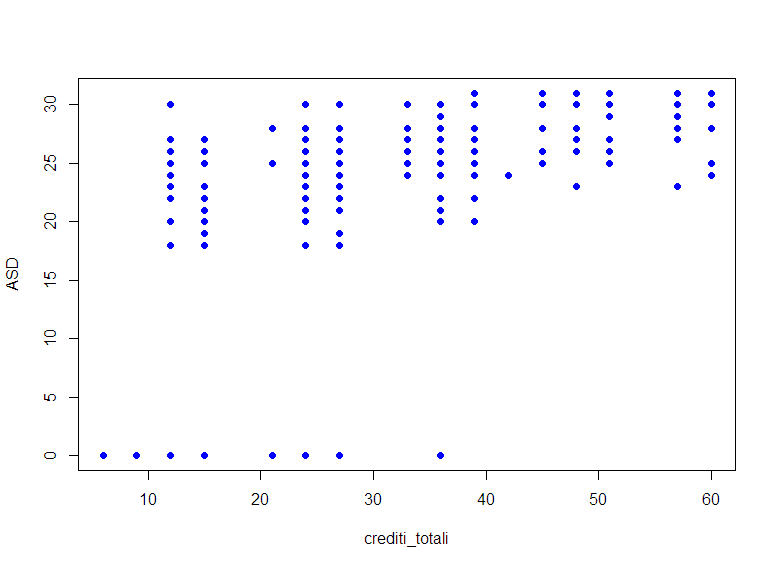
\includegraphics[width=\textwidth]{img/creditiAsd.png}
	\caption{Scatterplot tra Crediti totali e Algoritmi e strutture dati}
\end{figure}

\begin{figure}[H]
	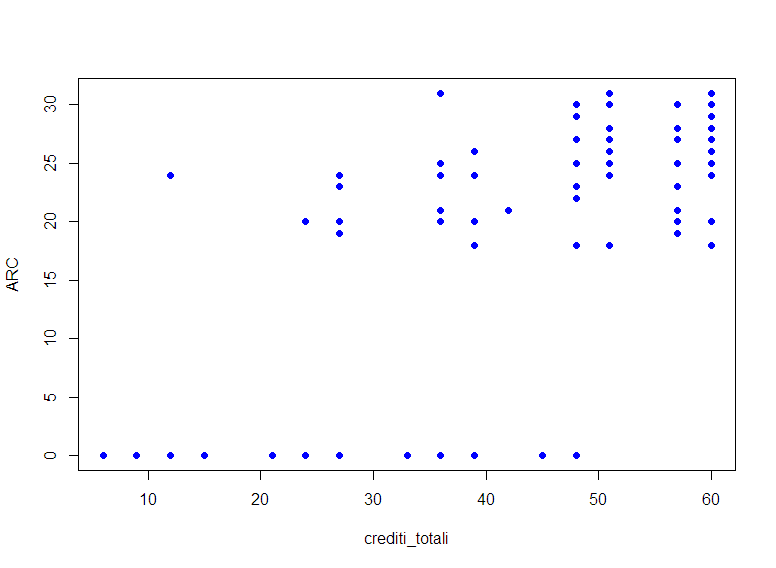
\includegraphics[width=\textwidth]{img/creditiArc.png}
	\caption{Scatterplot tra Crediti totali e Architetture degli elaboratori}
\end{figure}

L'attributo test è correlato maggiormente con l'attributo voto medio. 
Si può notare inoltre che il valore di correlazione è significativamente più alto di quello che l'attributo test ha con i voti dei singoli esami, con l'unica eccezione di MDL.
Questi valori lasciano suggerire che il punteggio conseguito al test d'ingresso di ogni studente sia un buon parametro per valutarne l'andamento generale piuttosto che i voti di un singolo esame.
Inoltre l'attributo test mostra una discreta correlazione con i crediti totali (e quindi anche con i crediti con voto).

Per quanto riguarda le correlazioni tra i voti dei diversi esami è possibile notare che il valore più alto è quello tra Architetture degli elaboratori e Programmazione che è circa pari a 0.43.
Mentre si ha una correlazione quasi nulla, ossia circa 0.10, tra il voto di Algoritmi e strutture dati e il voto di Analisi 1.

Nelle figure sono riportati gli scatterplot tra Architetture degli elaboratori e Programmazione e tra Algoritmi e strutture dati  e Analisi I.

\begin{figure}[H]
	\centering
	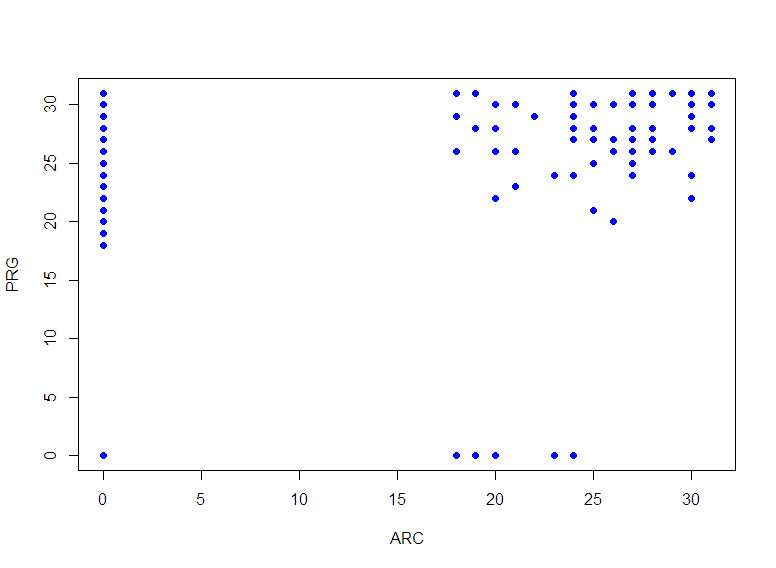
\includegraphics[width=\textwidth]{img/arcPrg.png}
	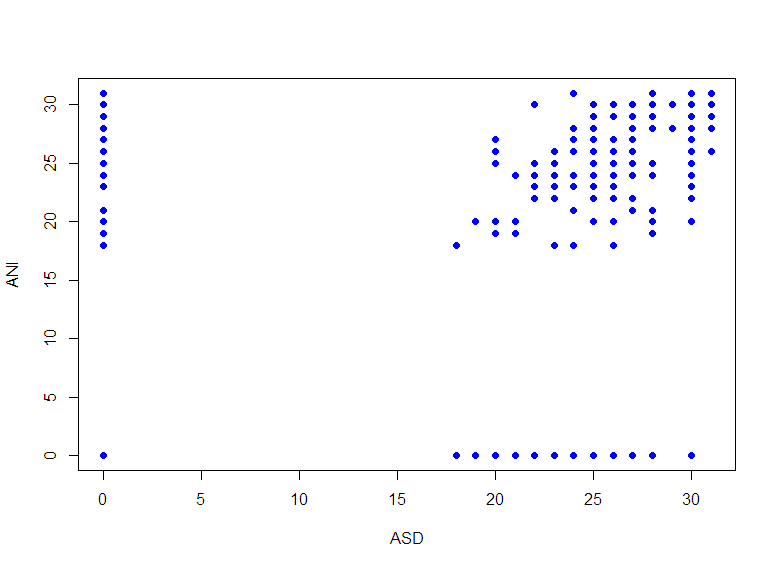
\includegraphics[width=\textwidth]{img/asdAni.png}
	\captionsetup{justification=centering}
	\caption{Scatterplot tra Architetture degli elaboratori e Programmazione e tra Algoritmi e strutture dati e Analisi I}
\end{figure}

\begin{figure}[H]
	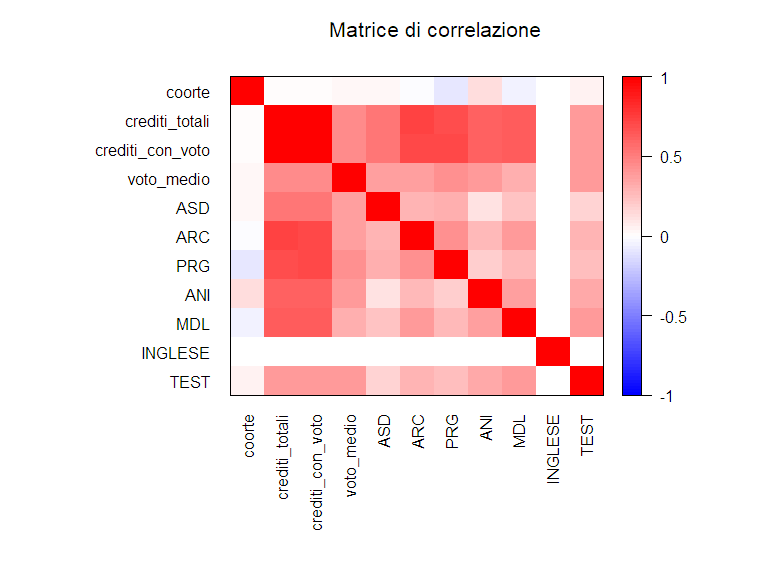
\includegraphics[width=\textwidth]{img/corMatrix.png}
	\caption{Matrice di correlazione}
	\label{fig:cMatrix}
\end{figure}

In Figura~\ref{fig:cMatrix} viene riportata la matrice di correlazione.
Per applicare gli algoritmi di clustering è stato utilizzato il software Weka. Tuttavia prima di applicare tali algoritmi è stato necessiaria un ulteriore fase di preprocessing
nella quale sono stati normalizzati tutti gli attributi del dataset in una scala di valori compresi tra zero e uno in modo da evitare problemi dovuto alle diverse scale di valori dei attributi.


\section{Clustering}
Come prima analisi mostriamo quella relativa ai tre attributi del dataset maggiormente correlati (a meno di correlazioni ovvie) ossia crediti totali, Architetture e Programmazione.
Infatti come è stato già precedentemente detto c'è una forte correlazione tra i crediti totali e architetture pari a 0.73 mentre tra crediti totali e Programmazione pari a 0.70.

È stato utilizzato l'algoritmo di Kmeans implementato in Weka specificando inizialmente un numero di cluster pari a due, lasciando i valori di default per la generazione dei centroidi.

In tabella \ref{c2AP} sono riportate le coordinate dei centroidi relativi all'esecuzione dell'algoritmo con un valore di k pari a 2.

% Cluster# 2 sse 51.35
% Attribute         Full Data          0          1
%                     (316.0)    (183.0)    (133.0)
% =================================================
% crediti_totali        0.496     0.6542     0.2782
% ARC                  0.2126     0.3295     0.0519
% PRG                  0.4929      0.851          0
% Clustered Instances
% 0      183 ( 58%)
% 1      133 ( 42%)

\begin{table}[ht]
	\centering
	\caption{Cluster k = 2 SSE 51.35}
	\label{c2AP}
	\begin{tabular}{@{}lllll@{}}
	\toprule
	  & Crediti totali & ARC  & PRG  & Istanze\\ \midrule
	0 & 0.65           & 0.32 & 0.85 & 183 ( 58\%)\\
	1 & 0.27           & 0.05 & 0    & 133 ( 42\%)\\ \bottomrule
	\end{tabular}
\end{table}

Come si può notare dalle cordinate dei centroidi questa prima esecuzione dell'algoritmo suddivide il dataset in due gruppi piuttosto distinti.
Il valore della somma degli errori al quadrato(SSE) in questa esecuzione è risultata pari a 51.53

In tabella \ref{c3AP} sono riportate le coordinate dei centroidi relativi all'esecuzione dell'algoritmo con un valore di k pari a 3.
% Cluster# 3 sse 14.85
% Attribute         Full Data          0          1          2
%                     (316.0)     (73.0)    (133.0)    (110.0)
% ============================================================
% crediti_totali        0.496      0.882     0.2782      0.503
% ARC                  0.2126     0.8259     0.0519          0
% PRG                  0.4929     0.8979          0     0.8199
% Clustered Instances
% 0       73 ( 23%)
% 1      133 ( 42%)
% 2      110 ( 35%)
\begin{table}[ht]
	\centering
	\caption{Cluster k = 3 SSE 14.85}
	\label{c3AP}
	\begin{tabular}{@{}lllll@{}}
	\toprule
	  & Crediti totali & ARC  & PRG  & Istanze\\ \midrule
	0 & 0.88           & 0.82 & 0.89 & 73 ( 23\%)\\
	1 & 0.27           & 0.05 & 0    & 133 ( 42\%)\\
	2 & 0.50           & 0    & 0.81 & 110 ( 35\%)\\ \bottomrule
	\end{tabular}
\end{table}

In questo caso il valore di SSE è pari a 14.8. È inoltre possibile constatare come l'algoritmo di kmean abbia messo in evidenza tre tipologie ben distinte di studenti:
\begin{itemize}
	\item Gli studenti appartenenti al cluster 0 sono gli studenti "migliori" avendo sostenuto la quasi totalità degli esami del primo anno alla fine della sessione estiva e riportando delle ottime valutazioni per quanto riguarda gli esami di Architetture e Programmazione;
	\item La seconda categoria di studenti (cluster 1) sono gli studenti "peggiori" che hanno sostenuto pochi esami e nel caso specifico delle materie considerate hanno conseguito valutazioni basse o non hanno sostenuto l'esame;
	\item Infine gli studenti appartenenti all'ultimo cluster sono gli studenti che hanno sostenuto Programmazione con un buon voto ma non hanno fatto l'esame di Architetture.
\end{itemize}
Come si evince andando ad analizzare i tre cluster in particolare notando le diverse combinazioni dei valori assunti dai centroidi dei voti, si capisce come sia assente la categoria di studenti che ha sostenuto con profitto l'esame di Architetture ma non ha sostenuto l'esame di Programmazione,
lasciando quindi intendere che se uno studente ha sostenuto l'esame di Architetture allora generalmente ha sostenuto con una buona valutazione l'esame di Programmazione.


% Cluster# 2 sse 12.4
% Attribute     Full Data          0          1
%                 (316.0)    (134.0)    (182.0)
% =============================================
% voto_medio       0.5684     0.3823     0.7054
% TEST             0.5996     0.4958      0.676
% Clustered Instances

% 0      134 ( 42%)
% 1      182 ( 58%)
\begin{table}[ht]
	\centering
	\caption{Cluster k = 2 SSE 12.4}
	\label{c2MT}
	\begin{tabular}{@{}lllll@{}}
	\toprule
	  & voto medio & Test  & Istanze\\ \midrule
	0 & 0.38       & 0.49  & 134 ( 42\%)\\
	1 & 0.70       & 0.67  & 182 ( 58\%)\\ \bottomrule
	\end{tabular}
\end{table}

La seconda analisi che è stata condotta riguarda gli attributi TEST e voto\_medio. E' stato scelto di analizzare 
questi due attributi congiuntamente in quanto, come è stato detto nel capitolo precedente, l'attributo voto\_medio 
presenta una buona correlazione con l'attributo TEST. 

In Tabella \ref{c3MT} sono riportate le coordinate dei centroidi relativi all'esecuzione dell'algoritmo con un numero di cluster pari a 3.
% Cluster# 3 sse 9.6
% Attribute     Full Data          0          1          2
%                 (316.0)     (85.0)    (146.0)     (85.0)
% ========================================================
% voto_medio       0.5684     0.3665     0.7529     0.4534
% TEST             0.5996     0.4188     0.6622     0.6729
% Clustered Instances

% 0       85 ( 27%)
% 1      146 ( 46%)
% 2       85 ( 27%)
\begin{table}[ht]
	\centering
	\caption{Cluster k = 3 SSE 9.6}
	\label{c3MT}
	\begin{tabular}{@{}lllll@{}}
	\toprule
	  & voto medio & Test  & Istanze\\ \midrule
	0 & 0.36       & 0.41  & 85  ( 27\%)\\
	1 & 0.75       & 0.66  & 146 ( 42\%)\\
	2 & 0.45       & 0.67  & 85  ( 27\%)\\ \bottomrule
	\end{tabular}
\end{table}

In questo caso è possibile notare come
l'algoritmo di k-means determini due cluster ben definiti che suddividono il dataset tra gli studenti che hanno una
media complessiva maggiore e un voto al test d'ingresso migliore e quelli che invece hanno una media più bassa e 
hanno conseguito punteggio basso al test di ingresso. Questi gruppi determinati sono coerenti con la correlazione 
che esiste tra i due attributi che tuttavia non è particolarmente elevata (diversamente dagli attributi presi in 
considerazione nell'analisi precedente). Infatti, oltre ai primi due cluster che identificano gli studenti "migliori"
e quelli "peggiori" esiste un terzo cluster di studenti che hanno conseguito un punteggio al test d'ingresso decisamente
positivo, ma non hanno mantenuto una media dei voti altrettanto buona. 
SSE in questo caso è 9.6

Infine l'ultima analisi che abbiamo deciso di condurre è quella relativa ai voti conseguiti dagli studenti del primo
anno durante la sessione estiva. In questo caso l'algoritmo di clustering è stato inizializzato con un valore di k=3.
In Tabella W sono riportate le coordinate dei centroidi al termine dell'algoritmo. In questo caso sono stati determinati
i profili di tre diversi gruppi di studenti:

\begin{itemize}
\item gli studenti che hanno conseguito una buona votazione negli esami di Algoritmi e Strutture Dati e Programmazione,
una votazione discreta all'esame di Analisi I e che non hanno sostenuto Matematica discreta e Logica e Architetture degli elaboratori;
\item gli studenti con le stesse caratteristiche del cluster precedente, ma che in più non hanno sostenuto Programmazione
\item gli studenti che hanno sostenuto tutti gli esami e con un buona votazione.
\end{itemize}

In Figura \ref{APC} è riportato lo scatter plot relativo ai voti di Architetture degli Elaboratori e Programmazione che sono
maggiormente correlati. Il valore del SSE in questo caso è pari a 106.19.
\begin{figure}[H]
	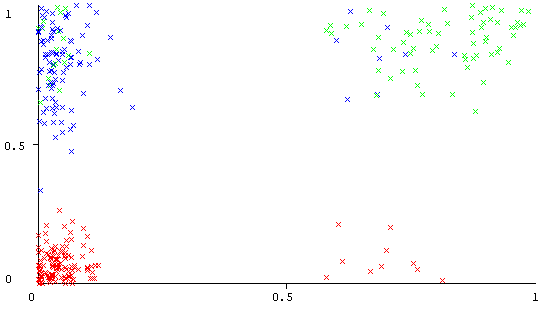
\includegraphics[width=\textwidth]{img/ARC-PRG-Cluster.png}
	\captionsetup{justification=centering}
	\caption{Scatter plot relativo ai cluster dei voti di Architetture degli Elaboratori e Programmazione}
	\label{APC}
\end{figure}

\section{Conclusioni}
In riferimento ai risultati ottenuti con le tecniche di clustering è possibile trarre le seguenti conclusioni riguardo
le carriere degli studenti:

\begin{itemize}
\item l'esame di Architetture degli Elaboratori risulta essere l'esame più difficile per gli studenti del primo anno,
  infatti la maggioranza non riesce a sostenerlo nel corso della sessione estiva. Tuttavia, generalmente gli studenti 
  che sostengono con profitto tale esame riescono a sostenere con profitto anche gli altri; 
\item la maggior parte degli studenti che ottengono un buon punteggio al test d'ingresso mantengono una buona media
  mentre quelli che hanno ottenuto un punteggio più basso hanno anche una media più bassa. Tuttavia è presente
  un significato gruppo di studenti che pur avendo ottenuto un buon punteggio al test di ingresso non riescono
  ad avere una media altrettanto buona;
\item La maggior parte degli studenti riesce a sostenere nel corso della sessione estiva gli esami di Algoritmi e 
  Strutture Dati, Analisi I e in alcuni casi l'esame di Programmazione con risultati altalenanti. Mentre 
  generalmente gli esami di Architetture degli Elaborati e Matematica Discreta e Logica non vengono sostenuti
  dagli studenti al termine del loro primo anno.
\end{itemize}

inoltre, in ciascuna delle analisi eseguite risultavano esserci almeno 3 gruppi di studenti che presentavano 
caratteristiche significativamente differenti.

\newpage 

\listoffigures
 
\newpage

% \thispagestyle{empty}\clearpage\mbox{}\clearpage

\listoftables

\newpage

% \thispagestyle{empty}\clearpage\mbox{}\clearpage

\end{document}